\documentclass{dtk}
\usepackage[ngerman]{babel}

\usepackage{
blindtext,
caption,
lmodern,
shortvrb,
tikz,
todonotes,
xltxtra
}

\newcommand{\taste}[1]{\makebox{\textsf{#1}}}
\catcode`\…=\active
\let…\dots % leider funktionieren die … nicht anders

\MakeShortVerb\|
\title{Neo \&\ \XeLaTeX\\Ergonomie und Zeichenvielfalt}
\author{Arno Trautmann}

\def\Paket#1{\textsf{#1}}
\def\LuaTeX{\textsf{Lua}\TeX}
\def\LuaLaTeX{\textsf{Lua}\LaTeX}

\begin{document}
\setmonofont[Scale=0.75]{DejaVu Sans Mono}
\address{Arno}{Trautmann}{Boxbergring 10\\ 69126 HD-Boxberg\\ |arno.trautmann@gmx.de|}
\maketitle
\begin{abstract}
Mit den Neuentwicklungen \XeTeX\ und \LuaTeX\ ist die \TeX-Welt in der Zeit von Unicode und modernen Schrifttechnologien angekommen. Doch das Haupteingabegerät, die Tastatur, ist bei vielen Benutzern größtenteils noch in der Zeit von mechanischen Schreibmaschinen steckengeblieben. In diesem Artikel soll das moderne Tastaturlayout Neo vorgestellt werden, das eine zeitgemäße Arbeit in der Textverarbeitung ermöglicht.
\end{abstract}
\section{Die Vergangenheit}
Seit den Anfängen des Maschinenschreibens hat sich an der Form und Belegung der Tastaturen wenig geändert: Die Form der Schreibmaschinentastatur wurde für Computer übernommen und seitdem fast nicht geändert. Minimale Anpassungen an einzelne Sprachen machten aus dem amerikanischen „\hbox{qwerty}“ (benannt nach der oberen Tastenreihe von links nach rechts gelesen) das deutsche „qwertz“ und das französische „azerty“. Aber warum sind die Tasten denn nun genau so angeordnet? Und warum sind sie so komisch schräg versetzt?

Die Antwort darauf liegt in der Vergangenheit: Im Jahre 1868 hat Christopher Latham Sholes ein Schreibmaschinenmodell mit der bekannten |qwerty|-Anordnung hergestellt. Die Versetzung der Tasten war aus rein mechanischen Gründen nötig, damit die Typenhebel für alle Buchstaben Platz fanden. Die häufigsten Buchstaben wurden halbkreisförmig angeordnet. Die restlichen Buchstaben wurden dazwischen verteilt; damit sich die Hebel nicht verkanten, musste darauf geachtet werden, dass häufig nacheinander angeschlagene Tasten (wie |qu|) nicht nebeneinander lagen. Das alles ergibt allerdings keine ergonomische Tastatur, die mit dem 10-Finger-System blind, schnell und angenehm zu bedienen ist, denn man muss recht häufig die Finger aus der Grundstellung bewegen, um die Tasten in der oberen oder unteren Reihe zu erreichen – z.\,B. das sehr häufige „e“ auf der oberen Reihe. Jede solche Bewegung bedeutet aber ein Verlust an Geschwindigkeit und mehr Arbeit für die Finger, was zu schnelleren Ermüdungserscheinungen führt und Gelenkschmerzen verursachen kann.

Schon im Jahre 1932 hat August Dvorak die ungeschickte Belegung als solche erkannt und nach längeren Studien eine neue Tastaturbelegung erstellt. Es folgten einige weitere Entwicklungen wie de-ergo und RISTOME, von denen sich aber bis heute keines durchgesezt hat. Das liegt einerseits am niedrigen Bekanntheitsgrad alternativer Layouts, andererseits am Problem des Umlernens: Selbst wenn man sich aufgerafft hat, eine neue Belegung zu erlernen (erfahrungsgemäß benötigt man ca. 2 Wochen, um wieder einigermaßen flüssig schreiben zu können), ist es immer ein Problem, an anderen Computern zu arbeiten – der Leser kennt dieses Problem vielleicht vom Umstieg von Word auf \LaTeX\ – eine Investition, die sich aber meist doch sehr gelohnt hat.

\subsection{Neo 1.0 und 1.1}
Im Jahre 2004 hat Hanno Behrens die erste Version von Neo veröffentlicht. Ca. ein Jahr später kam mit Neo 1.1 eine Verbesserung und teilweise Erweiterung des Layouts auf, z.\,B. wurde eine zweite \taste{Alt Gr}-Taste auf der linken Hand eingeführt, um den Zugriff auf Sonderzeichen zu vereinfachen.
\section{Gegenwart}
Seit dieser Zeit wird Neo 2.0 entwickelt (und steht kurz vor der Vollendung). Mit Version 2 wurden einige schwerwiegende Änderungen vorgenommen – die Tastenbelegung bleib zwar zu großen Teilen gleich, einige Buchstaben wurden auch wieder verlegt. Durch die Erfahrung beim alltäglichen Schreiben haben sich manche auf den ersten Blick guten Positionen und Kombinationen als ungünstig herausgestellt und wurden daher verbessert. Die aktuelle Belegung sieht folgendermaßen aus:
\begin{center}
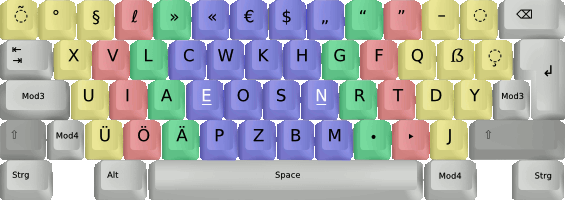
\includegraphics[width=.8\textwidth]{ebene2}
\captionof{figure}{Neo 2.0 – zweite Ebene mit Großbuchstaben}
\end{center}
Hauptänderung in Version 2.0 war jedoch die Einführung von „höheren Ebenen“ der Tastatur; insgesamt ist jede Taste sechsfach belegt: Ebene 1 sind die Zeichen, die durch direkten Anschlag erzeugt werden können (z.\,B. \taste{a}). Auf der Ebene 2 sind alle Zeichen, die durch Drücken von Shift (oder „Umschalt“) erzeugt werden. (z.\,B. Großbuchstaben \taste{A}, wenige Sonderzeichen \taste{§} und typographische Zeichen \taste{»« „“}) Ebene 3 wird durch \taste{Alt Gr} verwendet, was bei Neo 2 aber in \taste{Mod 3} umbenannt wurde. In dieser Ebene sind Sonderzeichen, die zum Programmieren verwendet werden, wie |\/{}_[ ]^!<>|.

Diese Funktionalität bieten fast alle Tastaturlayouts. Neo bietet aber noch eine vierte Ebene (dazu drückt man gleichzeitig \taste{Shift}, \taste{Mod 3} und z.\,B. \taste{a} und erhält ein \taste{$\alpha$}\footnote{Man gewöhnt sich sehr schnell an diese Kombinationen, ohne die Finger zu verrenken.}). Auf dieser sind größtenteils griechische Kleinbuchstaben. Diese Ebene ist \emph{nicht} dazu gedacht, griechischen Fließtext zu schreiben (denn dafür nimmt man ein griechisches Tastaturlayout), sondern für einzelne Buchstaben, etwa als Formelvariable.

\begin{center}
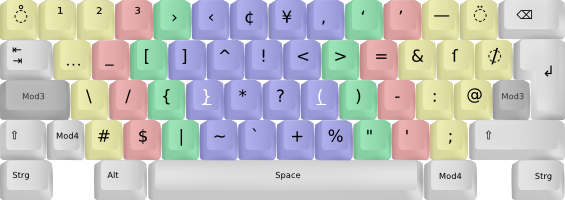
\includegraphics[width=.501\textwidth]{ebene3}%
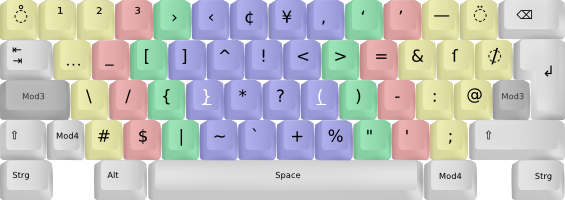
\includegraphics[width=.501\textwidth]{ebene3}
\captionof{figure}{Ebene 3 (Programmierzeichen), Ebene 4 (griechisch etc.)}
\end{center}

Ein völlig neues Konzept wurde mit der fünften Ebene in Neo eingeführt. Hierzu wurden zwei Tasten als \taste{Mod~4}\footnote{Ebene 3 \textrightarrow\ Mod 3, Ebene~4 \textrightarrow Mod~4. Shift/Umschalt fällt hier aus dem Namensschema raus.} definiert. Die Ebene~4 enthält neben einigen weiteren Sonderzeichen wie |•‣№| auch Steuerzeichen für die Arbeit am Text. Drückt man den rechten \taste{Mod~4}, so sind auf der linken Hand die Pfeiltasten und man kann im Text navigieren. Ebenso sind alle wichtigen Funktionen wie Enter, Löschen, Tabulator, Entfernen, Pos1, Ende, Einfügen, Bild hoch und Bild runter mit der linken Hand zu erreichen, ohne sie aus der Grundstellung zu bewegen. Bei einer normalen Tastatur müsste die rechte Hand einen Weg von bis zu 5cm zurücklegen, bis man an die Pfeiltasten kommt; der Weg zu Bild hoch ist meist noch länger und nur durch Draufschauen schnell zu finden. Das alles stört aber den Textfluss\footnote{Natürlich sollte man selten Entfernen/Löschen drücken – aber jeder macht Fehler!} und belastet die Arme durch die ständige weite Bewegung. Auf der rechten Tastaturhälfte findet sich auf der fünften Ebene eine Wiederholung des Ziffernblockes – alle Zahlen und Rechenzeichen sind somit in der Grundhaltung der Hand verfügbar und man muss weder die obere Zahlenreihe noch den „weit entfernten“ Zahlenblock verwenden. Zum Markieren kann wie gewohnt zusätzlich Shift gedrückt werden. Falls man viele Zahlen hintereinander eingeben muss oder sehr viel im Text (oder einem pdf z.\,B.) navigieren muss, ohne zu schreiben, ist der \taste{Mod~4}-Lock nützlich: Beide \taste{Mod~4} gleichzeitig gedrückt lassen die Funktion einrasten und man muss nicht ständig den Finger auf der Taste lassen. Das ist ganz analog zum bekannten CapsLock.

\begin{center}
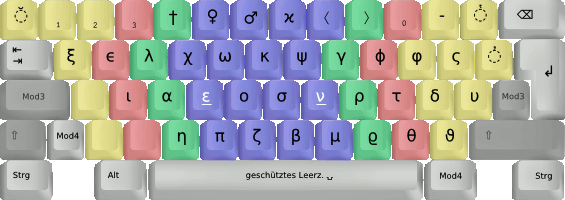
\includegraphics[width=.501\textwidth]{ebene5}%
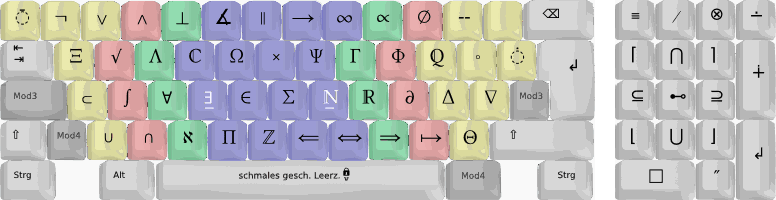
\includegraphics[width=.501\textwidth]{ebene6}
\captionof{figure}{Ebene~4: Steuerzeichen/Zahlen, Ebene 6: Sonderzeichen}
\end{center}

Schließlich bietet die Ebene 6, zu erreichen über \taste{Mod 3} und \taste{Mod~4}, noch eine weitere Vielfalt an Sonderzeichen, vor allem mathematischen Symbolen und einigen griechischen Großbuchstaben.

Nach dem gleichen Ebenensystem ist der Nummernblock belegt, der außer den Zahlen (erste Ebene) und den Steuerzeichen (vierte Ebene, redundant zu denen auf der fünften Ebene linke Hand) mathematische Relationen und Symbole enthält.

\subsection{Anordnung der Tasten}
Wie kann man sich denn nun all diese Tasten merken? Oft fällt es schon schwer, sich alle normalen Tasten zu merken, aber dann gleich 6 Zeichen pro Taste?

Hier hilft die sinngemäße Anordnung: Die Taste |a| hat die Zeichen |a A { α ⇣ ∀|. Vier davon kann man sich leicht merken. Weiterhin sind Zeichen wie |⇐⇔⇒| direkt nebeneinander angeordnet, sodass man sich nur die Position eines Zeichens merken muss und zwei weitere gleich findet. Es wird versucht, das Layout so zu gestalten, dass es sehr intuitiv verwendet werden kann und man kein „Raketentechniker“ sein muss, um es zu verstehen\footnote{Schon das Keyboarddesign „Space Cadett“ hatte genau dieses Problem.}

Dank der großen Zeichenvielfalt im Unicode reichen aber die sechs Tastaturebenen nicht aus, um alle mehr oder weniger häufig gebrauchten Zeichen abzudecken: Wie unter Linux und Sun OS bereits üblich, gibt es die Compose-Taste: Drückt man \taste{Mod 3} und Tabulator, danach (zwei) weitere Tasten, so werden diese sinngemäß „kombiniert“ und ergeben ein neues Zeichen. Die Eingabefolge \taste{Mod 3, Tabulator, a, e} ergibt das Zeichen \taste{æ}. Das klingt wiederum furchtbar kompliziert, doch wenn man das Zeichen oft benötigt, lohnt es sich, einmal in der Liste nachzusehen, wie es erzeugt wird und es dann stets direkt eingeben zu können, statt in einem Formeleditor o.\,ä. nachzuschlagen.

\subsection{Neo ist keine Tastatur…}
…\,sondern eine Tastaturbelegung. Neo orientiert sich an den Tasten einer handelsüblichen deutschen Tastatur. (Wie in den Abbildungen erkennbar.) Man muss lediglich einen Treiber installieren, der auf der Homepage verfügbar ist und meist nur ein oder zwei Klicks erfordert. Zur Zeit gibt es Treiber für Windows, Linux und Mac OS X\footnote{Wegen Softwareproblemen sind in Mac OS X momentan nur die ersten vier Ebenen verfügbar.}

Optimale Ergebnisse erhält man natürlich durch die Kombination einer ergonomischen Belegung und einer ergonomisch geformten Tastatur, z.\,B. Matrixtastaturen (PLUM) oder Konzepten wie DataHand.

\section{Neo, Unicode und \XeLaTeX}
Der \TeX-Nutzer wird sich nun fragen: „Na und? Die ganzen Zeichen kann ich auch als \TeX-Befehle über ASCII eingeben, da brauche ich weder Unicode noch \XeTeX\ und vor allem kein Neo.“ – Recht hat er. Aber damit wird der Quellcode ziemlich unleserlich. Wer ein |\"a| schöner findet als ein |ä| im Quellcode, muss diesen Artikel eigentlich nicht weiterlesen. Deutlich wird die bessere Lesbarkeit vor allem im Formelsatz, der meist nur schlecht auf einen Blick zu erfassen ist. Man vergleiche die beiden folgenden Eingaben:
\begin{verbatim}
  \[\int_{-\infty}^\infty d\Omega \left|\sqrt{\frac{3}{8\pi}}
                          \sin\theta e^{i\phi}\right|^2 \geq 0\]

  \[∫_{-∞}^∞ dΩ \left|√{\frac{3}{8π}} \sinϑ e^{iφ}\right|² ≥ 0\]
\end{verbatim}
% Für die Ausgabe der Formel mit dem angegeben Code – wir wollen ja nicht schummeln! Gut, ein wenig – kerning korrigiert.
\def\square{^2}
\catcode`\∫=\active
\catcode`\Ω=\active
\catcode`\√=\active
\catcode`\ϑ=\active
\catcode`\φ=\active
\catcode`\²=\active
\catcode`\≥=\active
\let∫\int
\letΩ\Omega
\let√\sqrt
\letϑ\theta
\letφ\phi
\let²\square
\let≥\geq
Mit wenigen kurzen Definitionen erhält man mit beiden Eingaben das gleiche Resultat:
  \[∫_{-∞}^∞\kern-1em dΩ \left\|√{\frac{3}{8π}} \sin ϑ e^{iφ}\right\|² ≥ 0\]
\catcode`\∫=12\catcode`\≥=12 %für die Verwendung in \verb
Zur Zeit muss man noch manuell definieren, dass |∫| wie ein |\int| behandelt wird und |≥| wie |\leq|, aber das (noch) experimentelle Paket \Paket{unicode-math} von Will Robertson wird hier Abhilfe schaffen.

Auch für typographisch korrekte Zeichen beim normalen Schreiben bietet Neo – in Kombination mit \XeLaTeX\footnote{Oder einem anderen unicodeartigen \TeX-System, etwa Λ, \LuaLaTeX\ oder \ConTeXt} – die Vorteile der direkten Eingabe. Man muss nicht mehr |--| schreiben, um den Halbgeviertstrich oder Gedankenstrich „–“ zu erhalten, sondern kann ihn einfach eingeben, ebenso der Geviertstrich oder englische Gedankenstrich: „—“ statt |---|. Auch Anführungszeichen, für die man mit \Paket{babel} |"` "'| schreiben muss (was ich mir noch nie merken konnte…), bietet die Tastatur „ “ sowie englische Anführungszeichen ” “ und französische » «. Die Auslassungspunkte, typographisch korrekt mit |\dots| statt |...| geschrieben, sind ebenso vorhanden…

Mit kurzen Definitionen kann man auch die üblichen \LaTeX-Umgebungen etwas „ungewohnt“, aber vielleicht übersichtlicher und einfacher schreiben:\footnote{Eine Definition, die sogar ohne \textsf{itemize} auskommt, wird im Paket \Paket{alttex} versucht.  \url{http://github.com/alt/alttex/tree/master}}
\small
\begin{verbatim}
\catcode`\•=\active      % Ab jetzt können • und ¹ als Befehle definiert werden
\catcode`\¹=\active      % 
\let•\item               % Die Zeichen • und ¹ bekommen
\let¹\item               % die gleiche Bedeutung wie \item
\end{verbatim}

\begin{minipage}{.4\textwidth}
\begin{verbatim}
\begin{itemize}
  • erster Punkt…
  •[2.] zweiter Punkt…
  •[⇒] es folgt der dritte Punkt…
\end{itemize} 
\end{verbatim}
\begin{verbatim}
\begin{enumerate}
  ¹ erster Punkt
  ¹ zweiter Punkt
\end{enumerate} 
\end{verbatim}
\end{minipage}
\catcode`\•=\active \let•\item
\catcode`\¹=\active \let¹\item
\hspace{1cm}\fbox{\begin{minipage}{.4\textwidth}
\ \\
\begin{itemize}
  • erster Punkt…
  •[2.] zweiter Punkt…
  •[\fontspec{DejaVu Sans Mono}⇒] es folgt der dritte Punkt…
\end{itemize}
\ \\
\begin{enumerate}
  ¹ erster Punkt
  ¹ zweiter Punkt
\end{enumerate}
\ \\
\end{minipage}}

\subsection{Besonderheiten}
Hier dürfen noch ein paar kleine Anmerkungen stehen, die den \TeX-Nutzer vielleicht im Besonderen freuen dürften:

In der DTK 3/2008 hat Markus Kohm berichtet, dass das große scharfe S normiert wurde – schon lange vor dieser Meldung stand bei Neo fest, dass der Buchstabe aufgenommen wird – leider gibt es nur sehr wenige Schriften, die das Zeichen besitzen… aber man kann es mit Neo direkt eingeben.

Für den Satz in gebrochenen Schriften ist sicher erfreulich, dass das lange s ebenfalls auf Neo vorhanden ist; mit einer richtig kodierten gebrochenen Schrift kann man also einfach „deutſch“ schreiben – auch in Antiqua natürlich.

Dank der vielen „toten Tasten“, also diakritischen Zeichen, sind alle Buchstaben aller europäischen, lateinisch basierten Alphabete schreibbar – optimal für vielsprachigen Satz.
\end{document}
